\documentclass[12pt, a4paper]{article}

\usepackage{import}
\usepackage{standalone}

\usepackage[top=4cm, right=2cm, bottom=2.7cm, left=2cm]{geometry}

\usepackage{wrapfig}
\usepackage{tabulary}
\usepackage{float}
\usepackage{pifont}
\usepackage{background}
\usepackage{tikz}


\pagestyle{empty}
\setlength{\parindent}{0pt}

\begin{document}
	\begin{minipage}{\textwidth}
		\section{Boomstammentransport \hfill\small Bron: Bebras}

			\begin{minipage}{0.6\linewidth}
				De bevers vervoeren stammen van het ene dorp naar het andere door ze de rivier af te laten drijven. Echter, om de rivieren niet te veel te versperren, vervoert elk dorp slechts stammen op één bepaalde dag van de week. In afwachting stockeren ze de stammen die ze van de andere dorpen hebben ontvangen.
				
				Het schema hiernaast stelt de kaart voor van de rivieren en geeft aan op welke dag van de week elk dorp stammen wil vervoeren. Zo wil dorp B bijvoorbeeld stammen naar dorpen E en F brengen, maar enkel op een zaterdag.
				
				Welke weg moeten de bevers volgen om zo snel mogelijk hun stammen van dorp A naar dorp H te brengen?
							
				\begin{table}[H]
					\centering
					\begin{tabular}{|c|c|}
						\hline
						\textbf{A} & A - B - E - H \\
						\textbf{B} & A - C - F - H \\ 
						\textbf{C} & A - B - F - H \\ 
						\textbf{D} & A - D - G - H \\
						\hline 
					\end{tabular}
				\end{table}
			\end{minipage} \hfill
			\begin{minipage}{0.34\linewidth}
					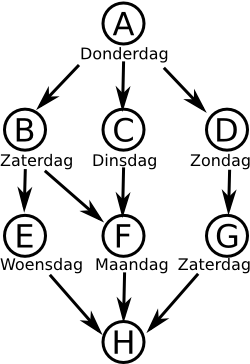
\includegraphics[width=\linewidth]{image1}
			\end{minipage}

	\end{minipage} \\ \\
		
\end{document}